\subsection{Домашка четвёртая}


\i 


\i Для начала заметим, что $(X_{n+1} = a | X_n = b)$ не зависит от $n$ (так как эта вероятность равна $P(\xi_{n+1} \modeq{4} a - b)$), поэтому $X_n$ будут
образовывать постоянную марковскую цепь, запишем её матрицу перехода 
    \[P_X = \begin{pmatrix}
        \frac{1}{7} & \frac{2}{7} & \frac{3}{7} & \frac{1}{7} \\ 
        \frac{1}{7} & \frac{1}{7} & \frac{2}{7} & \frac{3}{7} \\ 
        \frac{3}{7} & \frac{1}{7} & \frac{1}{7} & \frac{2}{7} \\ 
        \frac{2}{7} & \frac{3}{7} & \frac{1}{7} & \frac{1}{7}
    \end{pmatrix}\]


\i 
Рассмотрим координатную плоскость, где на оси $X$ будет откладывать координату первого передатчика, а на оси $Y$ --- второго. Тогда заметим, что должны выполняться
некоторые условия 
\begin{enumerate}
    \item $\frac{1}{4} + \frac{1}{3} \geq \abs{x - y} \geq \frac{1}{4} + \frac{1}{3} - \frac{1}{6}$, так как зоны передатчиков не должны перекрываться больше, чем на $\frac{1}{6}$, иначе 
        нам заведомо не хватит площади покрытия, и не могут стоять слишком далеко, иначе между ними будет пустое пространство (бирюзовая штриховка);
    \item $\frac{1}{4} - \frac{1}{6} \leq x \leq 1 + \frac{1}{6} - \frac{1}{4}$, так как первый передатчик не может стоять у края, иначе снова не хватит зоны покрытия
        (красная штриховка);
    \item $\frac{1}{3} - \frac{1}{6} \leq x \leq 1 + \frac{1}{6} - \frac{1}{3}$, аналогично со вторым пунктом. (зелёная штриховка).
\end{enumerate}
Таким образом мы получим следующую картинку:
\pgfplotsset{compat=1.15}
\usetikzlibrary{arrows}
\pagestyle{empty}
 

%<<<<<<<WARNING>>>>>>>
% PGF/Tikz doesn't support hatch filling very well
% Use PStricks for a perfect hatching export

\usetikzlibrary[patterns]
\definecolor{qqffqq}{rgb}{0,1,0}
\definecolor{ffqqtt}{rgb}{1,0,0.2}
\definecolor{qqaydv}{rgb}{0,0.6588235294117647,0.8352941176470589}
\definecolor{zzttqq}{rgb}{0.6,0.2,0}
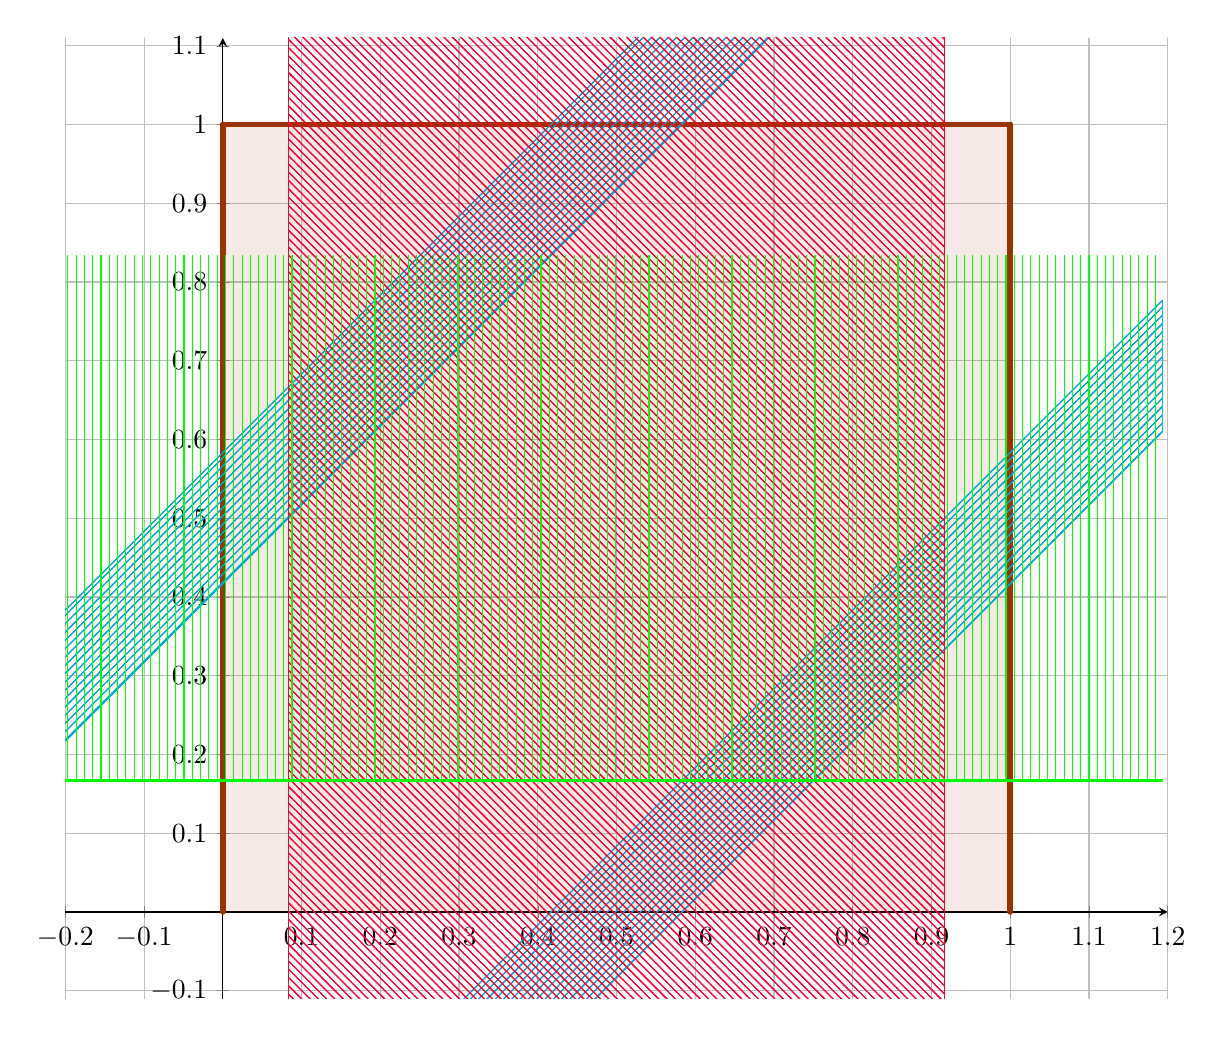
\begin{tikzpicture}[line cap=round,line join=round,>=triangle 45,x=1cm,y=1cm]
\begin{axis}[
x=10cm,y=10cm,
axis lines=middle,
ymajorgrids=true,
xmajorgrids=true,
xmin=-0.2,
xmax=1.2,
ymin=-0.11,
ymax=1.11,
xtick={-0.30000000000000004,-0.20000000000000004,...,1.3},
ytick={-0.1,0,...,1.2},]
\clip(-0.3261932561569772,-0.11133090811124503) rectangle (1.1934623633847328,1.205703962158231);
\fill[line width=2pt,color=zzttqq,fill=zzttqq,fill opacity=0.10000000149011612] (0,0) -- (1,0) -- (1,1) -- (0,1) -- cycle;
\draw [line width=2pt,color=zzttqq] (1,0)-- (1,1);
\draw [line width=2pt,color=zzttqq] (1,1)-- (0,1);
\draw [line width=2pt,color=zzttqq] (0,1)-- (0,0);
\draw[line width=0.4pt,color=qqaydv,fill=qqaydv,pattern=north east lines,pattern color=qqaydv](0.622370628824898,1.205703962158231)--(-0.3261932561569772,0.25714007717635595)--(-0.3261932561569772,0.09047341050968942)--(-0.32619325615697703,0.09047341050968957)--(0.7890372954915648,1.205703962158231);
\draw[line width=0.4pt,color=qqaydv,fill=qqaydv,pattern=north east lines,pattern color=qqaydv](1.1934623633847328,0.776795696718066)--(0.3053357585554218,-0.11133090811124488)--(0.47200242522208835,-0.11133090811124488)--(1.1934623633847328,0.6101290300513994)--(1.1934623633847328,0.776795696718066);
\draw[line width=0.4pt,color=qqaydv,fill=qqaydv,pattern=north east lines,pattern color=qqaydv](0.622370628824898,1.205703962158231)--(-0.3261932561569772,0.25714007717635595)--(-0.3261932561569772,0.09047341050968942)--(-0.32619325615697703,0.09047341050968957)--(0.7890372954915648,1.205703962158231);
\draw[line width=0.4pt,color=qqaydv,fill=qqaydv,pattern=north east lines,pattern color=qqaydv](1.1934623633847328,0.776795696718066)--(0.3053357585554218,-0.11133090811124488)--(0.47200242522208835,-0.11133090811124488)--(1.1934623633847328,0.6101290300513994)--(1.1934623633847328,0.776795696718066);
\draw[line width=0.4pt,color=ffqqtt,fill=ffqqtt,pattern=north west lines,pattern color=ffqqtt](0.08304733612311488,1.205703962158231)--(0.08304733612311488,-0.11133090811124503)--(0.9161918643806313,-0.11133090811124503)--(0.9161918643806313,1.205703962158231);
\draw[line width=0.4pt,color=ffqqtt,fill=ffqqtt,pattern=north west lines,pattern color=ffqqtt](0.08304733612311488,1.205703962158231)--(0.08304733612311488,-0.11133090811124503)--(0.9161918643806313,-0.11133090811124503)--(0.9161918643806313,1.205703962158231);
\draw[line width=1.2pt,color=qqffqq,fill=qqffqq,pattern=vertical lines,pattern color=qqffqq](-0.33952356860909744,0.8337882447440774)--(-0.33952356860909744,0.16727262213806735)--(1.206792675836853,0.16727262213806735)--(1.206792675836853,0.8337882447440774);
\draw[line width=1.2pt,color=qqffqq,fill=qqffqq,pattern=vertical lines,pattern color=qqffqq](-0.33952356860909744,0.8337882447440774)--(-0.33952356860909744,0.16727262213806735)--(1.206792675836853,0.16727262213806735)--(1.206792675836853,0.8337882447440774);
\end{axis}
\end{tikzpicture}\\
В силу независимости выбора $x$ и $y$ а также равновероятности всех выборов нам достаточно просто посчитать площадь двух трапеций, которые оказались заштрихованы 
трижды. Упустим скучные и тривиальные вычисления и скажем, что площадь одной трапеции равняется $\frac{1}{24}$, в силу симметрии тому же равняется и площадь 
второй трапеции, а значит вероятность того, что передатчиками будет покрыт весь отрезок составляем $\frac{2}{24} / 1 = \frac{2}{24}$.